% !TEX encoding = UTF-8
% !TEX program = pdflatex
% !TEX root = relazione-MEMOC.tex
% !TeX spellcheck = it_IT

\section{CPLEX} \label{sec:cplex}

Il modello CPLEX è stato implementato come specificato nella consegna della prima esercitazione con dei particolari accorgimenti per rendere il codice più comprensibile e manutenibile:

\begin{itemize}
	\item Le informazioni relative al problema e ad una sua possibile soluzione sono state modellate con due classi \texttt{Problem} e \texttt{Solution}. Inoltre, tutta la logica di risoluzione è stata incapsulata nella classe \texttt{CPLEXSolver}.
	\item Durante la dichiarazione delle variabili viene costruita una mappa di supporto per rendere più agevole l'utilizzo delle variabili all'interno dei vincoli. Viene inoltre limitato il numero di variabili, evitando di definire le variabili $x_{ii}$ e $y_{ii}$.
	\item I vincoli vengono definiti uno alla volta, in modo da semplificare la sintassi di definizione.
\end{itemize}

\subsection{Definizione delle variabili}

Le variabili in CPLEX, una volta create, vengono memorizzate in sequenza all'interno di un array interno al risolutore e l'unico modo per riferirsi ad una variabile è mediante la sua posizione nell'array interno.

Per riferirsi più facilmente alle variabili viene quindi creata una matrice di dimensione $N\times N$ che associa il ``\textit{nome della variabile}'' alla sua posizione interna nel risolutore.

\begin{lstlisting}[language=C++, caption=Creazione delle variabili $x_{ij}$]
// xMap[i][j] è una matrice N x N
for (int i = 0; i < N; ++i) {
	for (int j = 0; j < N; ++j) {
		if (i == j) continue;
		char htype = 'I';
		double obj = 0.0;
		double lb = 0.0;
		double ub = CPX_INFBOUND;
		snprintf(name, NAME_SIZE, "x_%d,%d", nodes[i], nodes[j]);
		char* xname = &name[0];
		CHECKED_CPX_CALL( CPXnewcols, env, lp, 1, &obj, &lb, &ub, &htype, &xname );
		xMap[i][j] = createdVars;
		createdVars++;
	}
}
\end{lstlisting}

\noindent La mappatura del nome viene fatta nella riga 12 del frammento di codice: \texttt{createdVars} è una variabile che tiene traccia del numero di variabili che sono state create nel risolutore e quindi la prossima variabile aggiunta avrà come indice interno il valore di \texttt{createdVars}. Il valore dell'indice viene quindi memorizzato nella mappa e poi incrementato, in modo che alla successiva iterazione dei ciclo questo sia ancora corretto.

Nello stesso frammento di codice è possibile osservare come \textbf{non} vengano create le variabili $x_{ii}$, questo perché quando i due indici sono uguali, l'\texttt{if} in riga 4 blocca l'esecuzione del corpo. 
Questa scelta è stata fatta perché tale variabile non è significativa per il problema, in quanto scegliere di spostare la trivella lungo l'arco $(i,i)$ equivale a lasciare ferma la trivella.
Quanto riportato è stato effettuato anche per le variabili $y_{ij}$.

\subsection{Definizione dei vincoli}

CPLEX permette di definire più vincoli con una sola istruzione, tuttavia la notazione per sfruttare questa possibilità è poco pratica da usare in quanto richiede che gli indici delle variabili e i corrispettivi coefficienti vengano passati come una matrice sparsa linearizzata in un vettore.
Se invece viene creato un vincolo alla volta, non c'è la necessità di gestire la matrice sparsa, in quanto questa è composta da una sola riga e quindi può essere considerata come vettore. 
Detto in altre parole, non è necessario utilizzare il vettore \texttt{rmatbeg} per tenere traccia dell'inizio delle varie righe, dato che essendoci un'unica riga, questa inizierà alla posizione 0 degli array utilizzati per definire il vincolo.

\begin{lstlisting}[language=C++, caption=Esempio di creazione di una serie di vincoli]
// Vincoli sul flusso in ingresso
for (int j = 0; j < N; ++j){
	std::vector<int> varIndex(N-1);
	std::vector<double> coef(N-1);
	int idx = 0;
	// Recupero gli indici dalla mappa delle varibaili
	for (int i = 0; i < N; ++i) {
		if (i==j) continue;
		varIndex[idx] = yMap[i][j];
		coef[idx] = 1;
		idx++;
	}
	char sense = 'E';
	double rhs = 1;
	snprintf(name, NAME_SIZE, "in_%d",j+1);
	char* cname = (char*)(&name[0]);

	int matbeg = 0;
	CHECKED_CPX_CALL( CPXaddrows, env, lp, 
						0, // Numero di variabili da creare
						1, // Numero di vincoli da creare
						varIndex.size(), // Numero di variabili nel vincolo con coeff != 0
						&rhs, // Parte destra del vincolo
						&sense, // Senso
						&matbeg, // 0 perché creo un solo vincolo
						&varIndex[0], // Inizio dell'array con gli indici delle variabili
						&coef[0], // Inizio dell'array con i coefficienti delle variabili
						NULL,  // Nomi per le nuove variabili
						&cname // Nome del vincolo
					);
}
\end{lstlisting}

\noindent Dal codice sopra riportato si può osservare come la chiamata della riga 19 definisce solamente un vincolo, pertanto per generare tutti vincoli del tipo

$$
\sum\limits_{j : (i,j) \in A} y_{ij} = 1 \quad \forall j \in N
$$

\noindent è necessario effettuare un iterazione esterna con il ciclo \texttt{for} di riga 2.

Questo modo di definire i vincoli potrebbe essere leggermente meno efficiente, dato che effettua più chiamate ai metodi del risolutore, ma l'impatto sulle prestazioni rimane comunque basso in quanto i vincoli vengono creati solamente all'inizializzazione del modello e il tempo necessario all'inizializzazione è comunque molto inferiore rispetto a quello necessario per l'ottimizzazione.

\subsection{Test del modello}

\`E stato richiesto di osservare qual'è la dimensione massima di un problema che il modello CPLEX riesce a risolvere entro un certo periodo di tempo.

Per fare ciò sono state prima generate 5 istanze casuali e 5 pseudo casuali per ogni dimensione $5$, $10$, $\ldots$, $100$ ed è stato eseguito CPLEX con un tempo limite di 10 minuti. Sono stati poi presi in considerazione 4 livelli di tempo limite: un secondo, dieci secondi, un minuto e dieci minuti ed è stato osservato qual'è la massima dimensione che può essere risolta entro tali vincoli.
I risultati medi delle esecuzioni sulle istanze di varie dimensioni sono riportati nella tabella \ref{tab:cplex-avg} e riassunti nel grafico \ref{fig:cplex-time}, mentre la corrispondenza tempo limite/difficoltà massima è riassunta nella tabella \ref{tab:cplex-recap}.

\begin{table}[htbp]
	\centering
	\resizebox{\textwidth}{!}{%
		\begin{tabular}{c|c|c|c|c|c|c|c|c|}
			\cline{2-9}
			\multicolumn{1}{l|}{} & \multicolumn{4}{c|}{\textbf{Pseudo}} & \multicolumn{4}{c|}{\textbf{Random}} \\ \hline
			\multicolumn{1}{|l|}{\textbf{Dimensione}} & \multicolumn{1}{l|}{\textbf{\begin{tabular}[c]{@{}l@{}}Tempo \\ medio\end{tabular}}} & \multicolumn{1}{l|}{\textbf{\begin{tabular}[c]{@{}l@{}}Tempo\\ minimo\end{tabular}}} & \multicolumn{1}{l|}{\textbf{\begin{tabular}[c]{@{}l@{}}Tempo\\ massimo\end{tabular}}} & \multicolumn{1}{l|}{\textbf{Fallimenti}} & \multicolumn{1}{l|}{\textbf{\begin{tabular}[c]{@{}l@{}}Tempo\\ medio\end{tabular}}} & \multicolumn{1}{l|}{\textbf{\begin{tabular}[c]{@{}l@{}}Tempo\\ minimo\end{tabular}}} & \multicolumn{1}{l|}{\textbf{\begin{tabular}[c]{@{}l@{}}Tempo\\ massimo\end{tabular}}} & \multicolumn{1}{l|}{\textbf{Fallimenti}} \\ \hline
			\multicolumn{1}{|c|}{5} & 0,02 & 0,01 & 0,04 & 0 & 0,02 & 0,01 & 0,04 & 0 \\ \hline
			\multicolumn{1}{|c|}{10} & 0,08 & 0,04 & 0,14 & 0 & 0,06 & 0,03 & 0,08 & 0 \\ \hline
			\multicolumn{1}{|c|}{15} & 0,14 & 0,06 & 0,23 & 0 & 0,20 & 0,09 & 0,31 & 0 \\ \hline
			\multicolumn{1}{|c|}{20} & 0,82 & 0,10 & 1,88 & 0 & 0,46 & 0,28 & 0,65 & 0 \\ \hline
			\multicolumn{1}{|c|}{25} & 1,38 & 0,17 & 3,88 & 0 & 0,92 & 0,43 & 1,57 & 0 \\ \hline
			\multicolumn{1}{|c|}{30} & 3,51 & 0,16 & 6,80 & 0 & 2,03 & 0,88 & 4,27 & 0 \\ \hline
			\multicolumn{1}{|c|}{35} & 4,75 & 0,52 & 11,94 & 0 & 3,87 & 1,47 & 6,87 & 0 \\ \hline
			\multicolumn{1}{|c|}{40} & 137,88 & 9,65 & 600,04 & 1 & 6,53 & 2,32 & 9,03 & 0 \\ \hline
			\multicolumn{1}{|c|}{45} & 31,50 & 5,01 & 94,31 & 0 & 10,22 & 9,11 & 12,89 & 0 \\ \hline
			\multicolumn{1}{|c|}{50} & 114,99 & 18,88 & 350,22 & 0 & 18,16 & 13,72 & 24,37 & 0 \\ \hline
			\multicolumn{1}{|c|}{55} & 36,53 & 26,39 & 47,00 & 0 & 24,98 & 15,83 & 53,49 & 0 \\ \hline
			\multicolumn{1}{|c|}{60} & 52,91 & 28,03 & 77,75 & 0 & 42,82 & 23,03 & 73,45 & 0 \\ \hline
			\multicolumn{1}{|c|}{65} & 215,51 & 55,89 & 600,08 & 1 & 81,70 & 62,26 & 119,60 & 0 \\ \hline
			\multicolumn{1}{|c|}{70} & 196,50 & 60,60 & 600,08 & 1 & 62,39 & 35,62 & 91,72 & 0 \\ \hline
			\multicolumn{1}{|c|}{75} & 239,86 & 6,97 & 411,80 & 0 & 90,25 & 48,40 & 114,86 & 0 \\ \hline
			\multicolumn{1}{|c|}{80} & 318,38 & 57,05 & 600,10 & 2 & 203,84 & 89,87 & 399,65 & 0 \\ \hline
			\multicolumn{1}{|c|}{85} & 245,64 & 93,26 & 600,14 & 1 & 268,20 & 69,19 & 550,24 & 0 \\ \hline
			\multicolumn{1}{|c|}{90} & 474,56 & 207,08 & 600,17 & 3 & 311,61 & 155,87 & 600,13 & 1 \\ \hline
			\multicolumn{1}{|c|}{95} & 517,15 & 185,08 & 600,20 & 4 & 445,41 & 238,19 & 600,20 & 1 \\ \hline
		\end{tabular}%
	}
	\caption{Risultatati medi dell'esecuzione del risolutore CPLEX su 5 istanze diverse per ogni dimensione. Tutti i tempi riportati nella tabella sono espressi in secondi.}
	\label{tab:cplex-avg}
\end{table}

\begin{figure}[htbp]
	\centering
	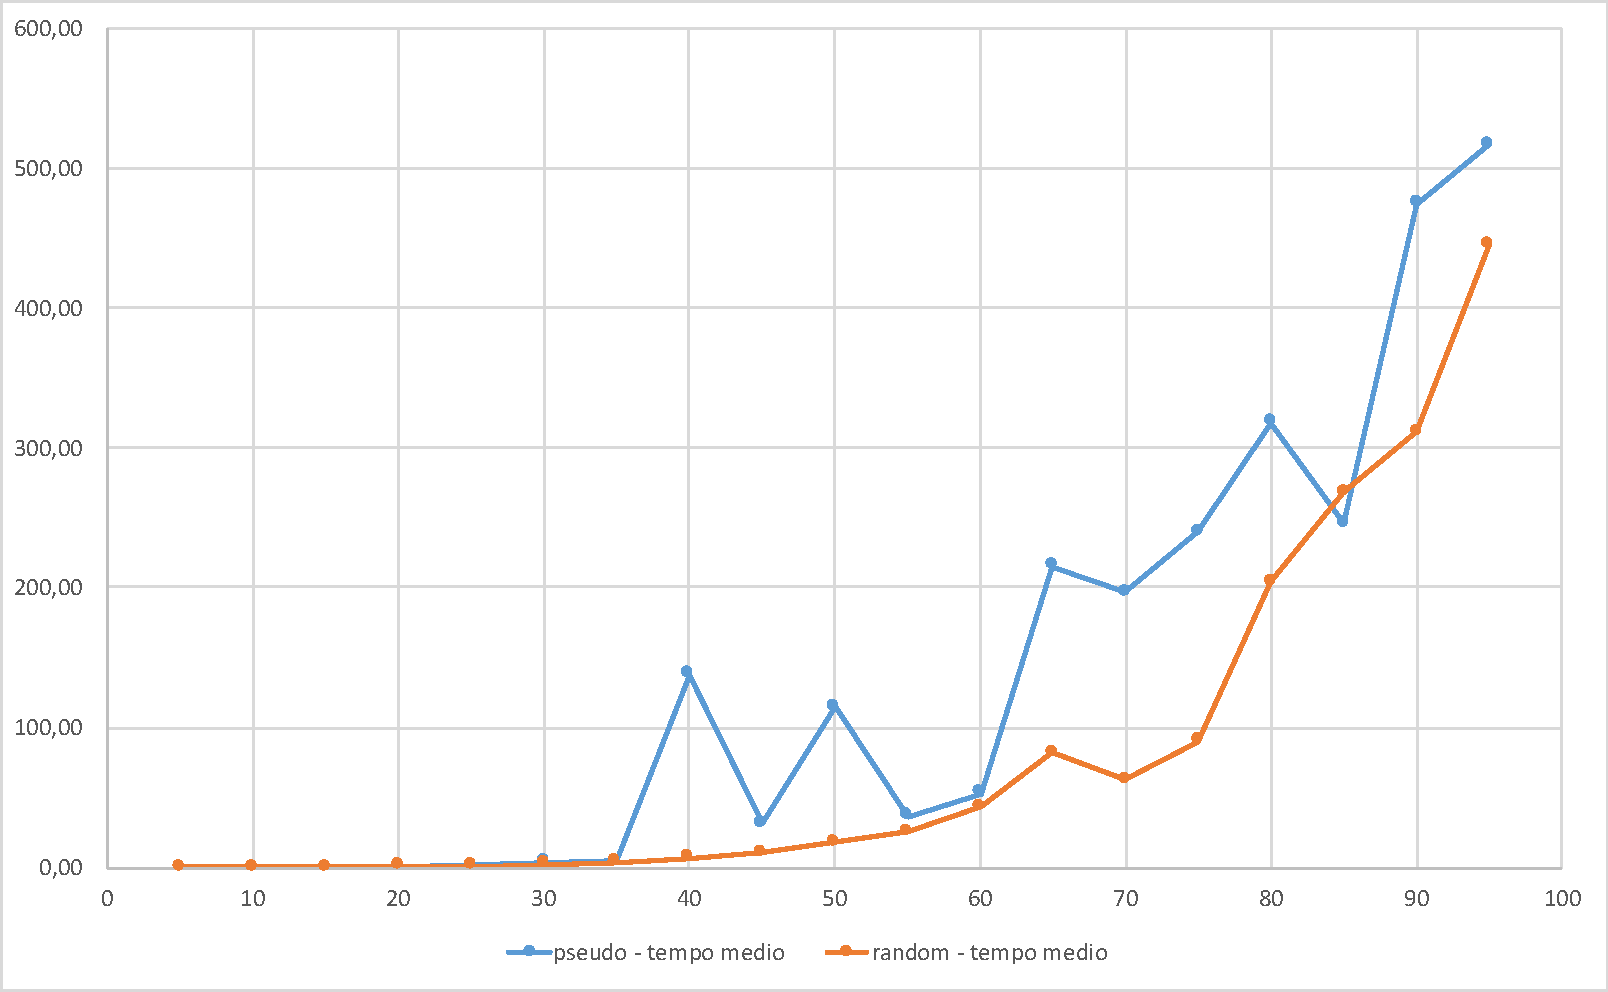
\includegraphics[width=\textwidth]{immagini/cplex-time.pdf}
	\caption{Tempo medio impiegato da CPLEX per risolvere le varie istanze}\label{fig:cplex-time}
\end{figure}

\begin{table}[htbp]
	\centering
	\begin{tabular}{c|c|c|}
		\cline{2-3}
		& \multicolumn{2}{c|}{\textbf{Dimensione}} \\ \hline
		\multicolumn{1}{|c|}{\textbf{Time limit} (s)} & \textbf{Pseudo}      & \textbf{Rand}     \\ \hline
		\multicolumn{1}{|c|}{1}                   & 20                   & 25                \\ \hline
		\multicolumn{1}{|c|}{10}                  & 35                   & 45                \\ \hline
		\multicolumn{1}{|c|}{60}                  & 60                   & 60                \\ \hline
		\multicolumn{1}{|c|}{600}                 & 85                   & 95               \\ \hline
	\end{tabular}
	\caption{Massima difficoltà mediamente risolvibile entro i rispettivi limiti temporali. Per determinare la difficoltà è stata usata la media, senza prendere in considerazione i casi limite in cui già per $N$ bassi non viene trovata una soluzione.}
	\label{tab:cplex-recap}
\end{table}

Dai risultati ottenuti si può osservare che:

\begin{itemize}
	\item Le istanze generate casualmente sembrano essere mediamente più facili da risolvere rispetto a quelle generate in modo pseudo casuale.
	\item Per quanto riguarda le istanze pseudo casuali, già con $N=40$ è stata trovata un'istanza che CPLEX non riesce a risolvere entro 10 minuti d'esecuzione.
	\item Con $N = 100$ solo due istanze di quelle generate casualmente sono state risolte, mentre di quelle pseudo casuali non ne è stata risolta nessuna. 
	Pertanto sembra che la distribuzione dei punti sia piuttosto influente sulle prestazioni dell'algoritmo.
\end{itemize}
